% Solution: Tadelis (2013) Exercise 8.5 "Technology Adoption". Input by \solitem.
% New in the 30-item list. Check: check_B_L03.py.
\begin{exsol}{Tadelis Exercise 8.5}{170}{Exam}{3}
\asked (a) Tree, Nash and subgame-perfect equilibria of the simultaneous task/training game;
(b) tree and number of proper subgames once the CEO first decides whether to adopt (outside
payoff $(1,1)$); (c) Nash and subgame-perfect equilibria of that larger game.

\method Simultaneous moves as an information set (Lecture~3, slides~22--23; Tadelis Def.~7.2,
p.~135); mixed equilibria by the principle of indifference (Lecture~3, slides~10--12); proper
subgames (Lecture~4, slides~14--16; Tadelis Def.~8.2, p.~154, which counts the whole game); SPE
by replacing the subgame with each of its Nash equilibria and optimizing at the root
(Lecture~4, slide~17; Tadelis \S8.2, Def.~8.3, p.~157). The structure is the voluntary battle of
the sexes (Lecture~3, slide~36; Lecture~4, slide~19; Tadelis pp.~154--159).

\solution
\textbf{Notation.} CEO = player~1 ($H$ or $L$), manager = player~2 ($G$ or $B$); in (b) the CEO
first chooses $N$ (no adoption) or $A$ (adopt). $p = \Pr_1(H)$, $q = \Pr_2(G)$ in the
simultaneous game.

\textbf{(a) Tree and equilibria of the simultaneous game.}
\begin{center}
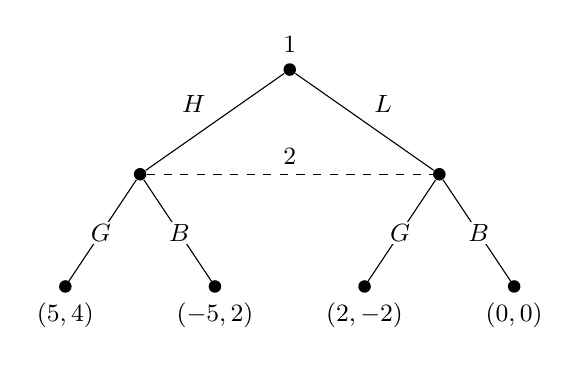
\begin{tikzpicture}[scale=0.95,dot/.style={circle,fill,inner sep=1.6pt},
  every node/.style={font=\small}]
  \node[dot,label=above:{1}] (x) at (0,0) {};
  \node[dot] (h) at (-2,-1.4) {};
  \node[dot] (l) at (2,-1.4) {};
  \draw (x) -- node[above left] {$H$} (h);
  \draw (x) -- node[above right] {$L$} (l);
  \draw[dashed] (h) -- node[above] {2} (l);
  \foreach \xx/\p/\lab/\pay in {-3/h/$G$/{$(5,4)$}, -1/h/$B$/{$(-5,2)$},
                               1/l/$G$/{$(2,-2)$}, 3/l/$B$/{$(0,0)$}} {
    \node[dot,label=below:{\pay}] at (\xx,-2.9) {};
    \draw (\p) -- node[fill=white,inner sep=1pt] {\lab} (\xx,-2.9);
  }
\end{tikzpicture}
\end{center}
\emph{Pure:} best replies $BR_1(G) = H$ ($5 > 2$), $BR_1(B) = L$ ($0 > -5$), $BR_2(H) = G$
($4 > 2$), $BR_2(L) = B$ ($0 > -2$). Pure equilibria: $(H, G)$ with $(5,4)$ and $(L, B)$ with $(0,0)$.

\emph{Mixed:} the manager is indifferent when
\begin{equation}
  u_2(G) = 4p - 2(1-p) \;=\; 2p + 0\cdot(1-p) = u_2(B) \;\Rightarrow\; 6p - 2 = 2p
  \;\Rightarrow\; p = \tfrac12 , \label{eq:tadelis-8-5-p}
\end{equation}
and the CEO is indifferent when
\begin{equation}
  u_1(H) = 5q - 5(1-q) \;=\; 2q + 0\cdot(1-q) = u_1(L) \;\Rightarrow\; 10q - 5 = 2q
  \;\Rightarrow\; q = \tfrac58 . \label{eq:tadelis-8-5-q}
\end{equation}
Payoffs in the mixed equilibrium: $u_1 = 2q = \frac54$, $u_2 = 2p = 1$.

\emph{Subgame perfection:} the only proper subgame is the game itself (player~2's nodes share an
information set, so no subgame starts at them). Every Nash equilibrium is therefore subgame
perfect: $(H,G)$, $(L,B)$ and $(\frac12 H + \frac12 L,\ \frac58 G + \frac38 B)$.

\textbf{(b) The entire game.} The CEO moves first at $x_0$: $N$ ends the game with $(1,1)$; $A$
leads to $x_1$, where the game of (a) is played.
\begin{center}
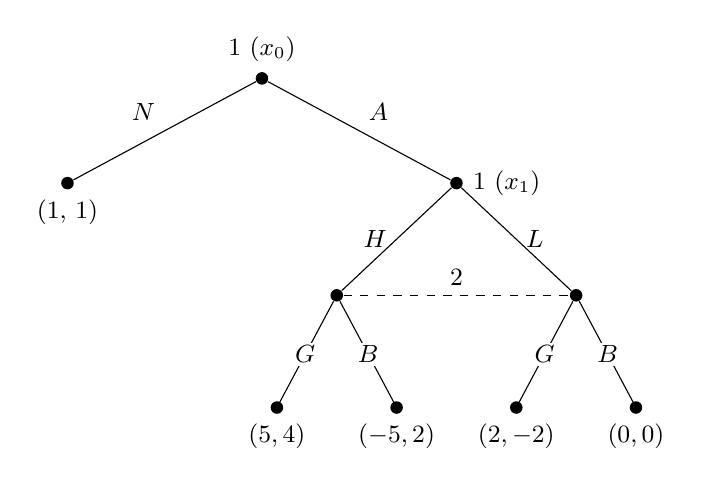
\begin{tikzpicture}[scale=0.95,dot/.style={circle,fill,inner sep=1.6pt},
  every node/.style={font=\small}]
  \node[dot,label=above:{1 ($x_0$)}] (r) at (0,0) {};
  \node[dot,label=below:{$(1,\,1)$}] (n) at (-2.6,-1.4) {};
  \node[dot,label=right:{1 ($x_1$)}] (x1) at (2.6,-1.4) {};
  \draw (r) -- node[above left] {$N$} (n);
  \draw (r) -- node[above right] {$A$} (x1);
  \node[dot] (h) at (1.0,-2.9) {};
  \node[dot] (l) at (4.2,-2.9) {};
  \draw (x1) -- node[left] {$H$} (h);
  \draw (x1) -- node[right] {$L$} (l);
  \draw[dashed] (h) -- node[above] {2} (l);
  \foreach \xx/\p/\lab/\pay in {0.2/h/$G$/{$(5,4)$}, 1.8/h/$B$/{$(-5,2)$},
                               3.4/l/$G$/{$(2,-2)$}, 5.0/l/$B$/{$(0,0)$}} {
    \node[dot,label=below:{\pay}] at (\xx,-4.4) {};
    \draw (\p) -- node[fill=white,inner sep=1pt] {\lab} (\xx,-4.4);
  }
\end{tikzpicture}
\end{center}
Candidate roots of proper subgames are singleton information sets: $x_0$ and $x_1$. Player~2's
nodes are excluded (each would cut her information set). So there are \textbf{two proper
subgames}: the whole game and the adoption subgame starting at $x_1$ (one, if the whole game is
not counted, as in Gibbons).

\textbf{(c) Equilibria of the entire game.} The CEO now has two information sets. His
strategies are $S_1 = \{NH, NL, AH, AL\}$; the manager's are $S_2 = \{G, B\}$.
\begin{center}
\begin{tabular}{r|c|c|}
\multicolumn{1}{r}{} & \multicolumn{1}{c}{$G$} & \multicolumn{1}{c}{$B$}\\ \cline{2-3}
$NH$ & $1,\ \br{1}$ & $\br{1},\ \br{1}$ \\ \cline{2-3}
$NL$ & $1,\ \br{1}$ & $\br{1},\ \br{1}$ \\ \cline{2-3}
$AH$ & $\br{5},\ \br{4}$ & $-5,\ 2$ \\ \cline{2-3}
$AL$ & $2,\ -2$ & $0,\ \br{0}$ \\ \cline{2-3}
\end{tabular}
\end{center}
\emph{Pure Nash equilibria:} $(AH, G)$, $(NH, B)$, $(NL, B)$.

\emph{All Nash equilibria.} Given $q$, the CEO's payoffs are $1$ ($NH$, $NL$), $5q - 5(1-q) = 10q - 5$
($AH$) and $2q$ ($AL$). The manager's gain from $G$ over $B$ is $0$ against $N\cdot$, $+2$ against
$AH$ and $-2$ against $AL$.
\begin{itemize}
  \item $q < \frac12$: $1 > 2q$ and $1 > 10q - 5$, so the CEO plays $N$ (any mix of $NH$, $NL$); the
  manager is never reached and any $q$ is a best reply. \emph{Equilibria.}
  \item $q = \frac12$: $N$ and $AL$ tie at 1 ($AH$ gives 0). For $0 < q < 1$ the manager must be
  indifferent, i.e.\ $-2\Pr(AL) = 0$: the CEO stays on $N$. \emph{Equilibria.}
  \item $\frac12 < q < \frac58$: $AL$ is the unique best reply ($2q > 1$, $2q > 10q - 5$); then the
  manager strictly prefers $B$, $q = 0$. Contradiction.
  \item $q = \frac58$: $AH$ and $AL$ tie at $\frac54 > 1$; the manager is indifferent iff
  $2\Pr(AH) - 2\Pr(AL) = 0$, i.e.\ $\frac12 AH + \frac12 AL$. \emph{Equilibrium.}
  \item $\frac58 < q \le 1$: $AH$ is the unique best reply; then the manager plays $G$, $q = 1$.
  \emph{Equilibrium} $(AH, G)$ at $q = 1$ only.
\end{itemize}
So the Nash equilibria are
\[
  \bigl\{(\text{any mix of } NH, NL;\ q) : q \le \tfrac12\bigr\}
  \cup \bigl\{(\tfrac12 AH + \tfrac12 AL;\ \tfrac58)\bigr\}
  \cup \bigl\{(AH;\ G)\bigr\}.
\]

\emph{Subgame-perfect equilibria.} In the adoption subgame play must be one of its three Nash
equilibria; replace $x_1$ by its value and optimize at $x_0$:
\begin{center}
\begin{tabular}{lccl}
\toprule
Subgame equilibrium & Value $(u_1,u_2)$ & CEO at $x_0$ & SPE \\
\midrule
$(H, G)$ & $(5, 4)$ & $A$ ($5 > 1$) & $(AH, G)$, payoffs $(5,4)$ \\
$(L, B)$ & $(0, 0)$ & $N$ ($1 > 0$) & $(NL, B)$, payoffs $(1,1)$ \\
$(\frac12, \frac58)$ & $(\frac54, 1)$ & $A$ ($\frac54 > 1$) & $(A,\ \frac12 H + \frac12 L;\ \frac58 G)$, payoffs $(\frac54, 1)$ \\
\bottomrule
\end{tabular}
\end{center}
Three SPE. The Nash equilibria that are not subgame perfect are $(NH, B)$ and every profile of the
first family other than $(NL, B)$: after adoption they prescribe $(H, B)$ or $(L, q)$ with
$q > 0$, or a mix of $H$ and $L$ that is not $\frac12$--$\frac12$ with $q \le \frac12$, none of
which is a Nash equilibrium of the subgame. For instance, in $(NH, B)$ the CEO's plan $H$ against
$B$ gives him $-5 < 0$.

\interp Whether a new technology is adopted depends on what each side expects the other to do
after adoption, not only on its potential ($5,4$). If the CEO expects the manager to train badly
he does not adopt, and the expectation is self-fulfilling. Adoption has an option value only if
the subgame is expected to coordinate on $(H,G)$, or at least on the mixed play, which gives
$\frac54 > 1$. The outside option $(1,1)$ works like the UK's no-deal option in the Brexit case
(Lecture~4, slide~11): it sets the bar that the continuation must clear, and it eliminates the
$(H,B)$ plan, which no rational CEO would carry out after adopting.

\verify \texttt{check\_B\_L03.py} finds the pure equilibria of the subgame, solves
\eqref{eq:tadelis-8-5-p}--\eqref{eq:tadelis-8-5-q} with sympy, checks the mixed profile and its
payoffs $(\frac54, 1)$ exactly, finds the pure equilibria $(NH,B)$, $(NL,B)$, $(AH,G)$ of the
$4\times2$ matrix, scans $q$ on a grid of step $\frac1{160}$ plus $\frac12, \frac35, \frac58$
(equilibria exactly at $q \le \frac12$, $q = \frac58$, $q = 1$), and replaces the subgame by each
equilibrium value to get the three SPE. Output line: \texttt{tadelis-8-5: subgame NE (H,G), (L,B),
(1/2, 5/8); three SPE}. Tadelis prints no answer.

\mistakes
\begin{itemize}
  \item Treating $(NH, B)$ and $(NL, B)$ as the same equilibrium: they are different strategies,
  and only $(NL, B)$ is subgame perfect.
  \item Forgetting the mixed equilibrium of the subgame, and with it the third SPE (adoption with
  mixed play).
  \item Saying the game of (a) has subgames at player~2's nodes; they belong to one information
  set.
\end{itemize}

\answer{(a) Nash (all subgame perfect, since the only subgame is the game itself): $(H,G)$, $(L,B)$,
$(\frac12 H + \frac12 L,\ \frac58 G + \frac38 B)$ with payoffs $(5,4)$, $(0,0)$, $(\frac54, 1)$.
(b) Tree above; two proper subgames (the whole game and the post-adoption game). (c) Pure Nash:
$(AH,G)$, $(NH,B)$, $(NL,B)$; all Nash: $N$ (any mix of $NH$, $NL$) with $\Pr(G) \le \frac12$,
$(\frac12 AH + \frac12 AL, \frac58)$, $(AH, G)$. SPE: $(AH, G)$, $(NL, B)$ and
$(A, \frac12 H + \frac12 L;\ \frac58 G)$.}
\end{exsol}
